% Chapter 6

\chapter[Video Tracking System]{Video Tracking System} % Main chapter title

\label{Chapter6} % For referencing the chapter elsewhere, use \ref{Chapter6} 

%----------------------------------------------------------------------------------------

\section{Overview}
In order to implement the augmented reality visualisation element of the system, and satisfy the related objectives, a live video feed of the swarm was needed. A method for tracking the positions of each individual robot in the swarm based on images from this feed was also required. Prior to the start of the project the YRL already had infrastructure in place for this kind of task, in the form of a machine vision camera placed above an 'arena', and software for processing the output of this camera using the `ARuCo\cite{Garrido:2014}' fiducial marker based tracking system. Figure \ref{fig:CameraLayout} shows the arrangement of the machine vision camera used for robot tracking, and the robot arena. It was determined that incorporating this existing infrastructure into the system was the quickest way to get this required aspect of the system working, allowing work to focus on the novel aspects sooner.

\begin{figure}
	\centering
	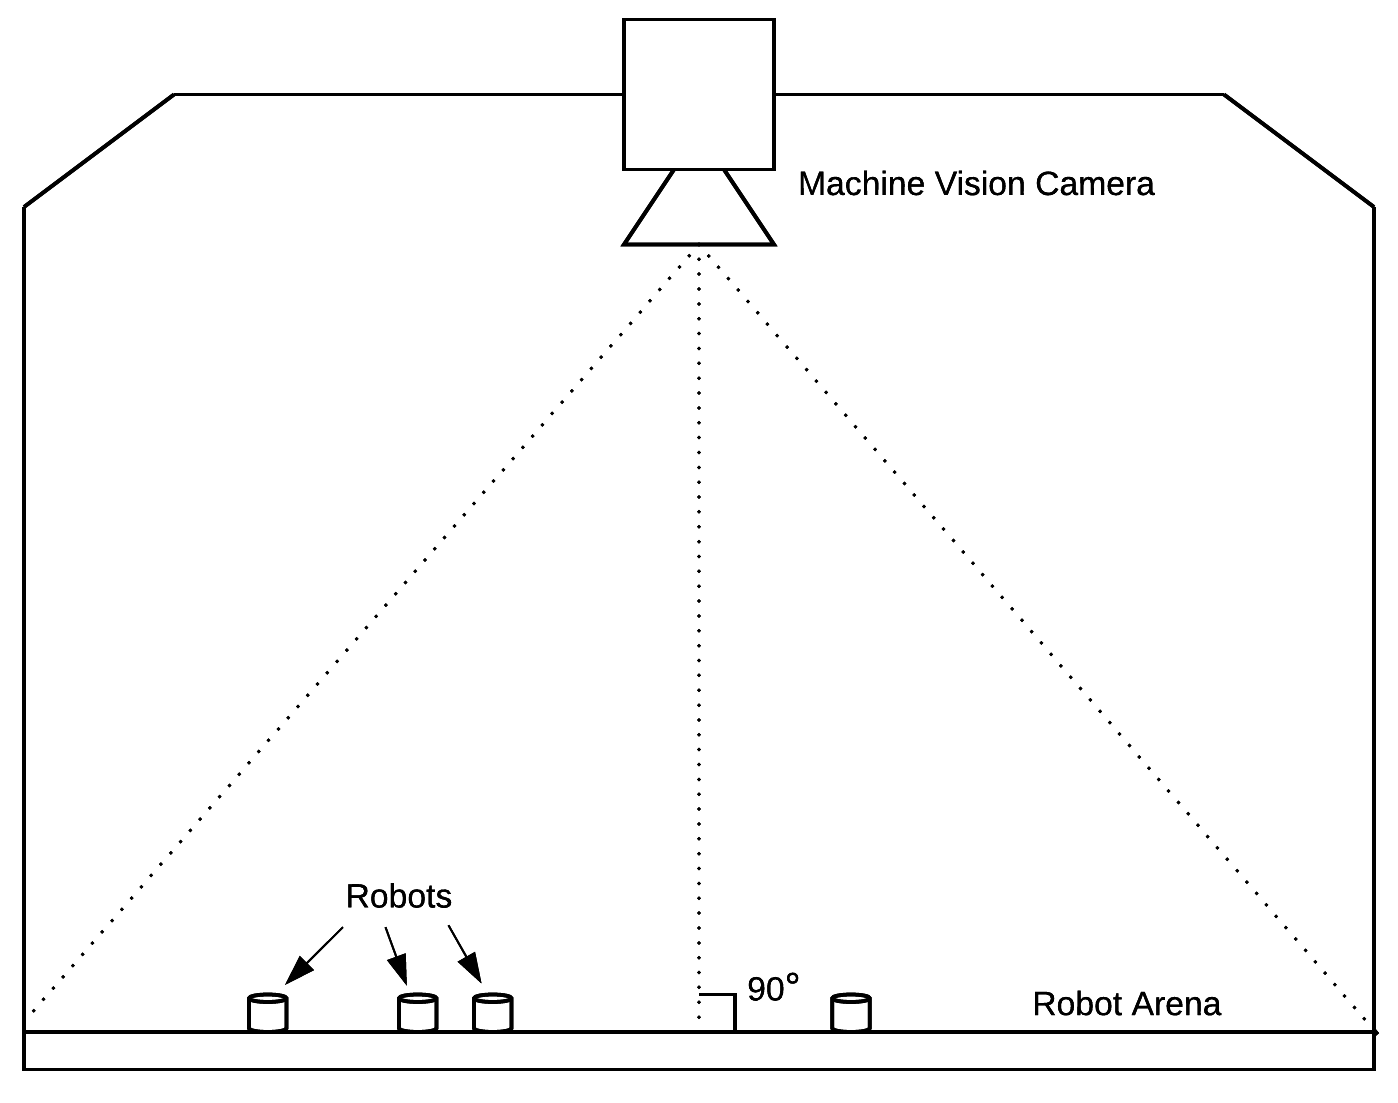
\includegraphics[scale=0.3]{Figures/CameraLayout.png}
	\decoRule
	\caption[Tracking Camera Arrangement]{Arrangement of the tracking camera over the robot arena.}
	\label{fig:CameraLayout}
\end{figure}

%----------------------------------------------------------------------------------------

\section{Camera}
[WHAT CAMERA IS USED? DETAILS.]


%----------------------------------------------------------------------------------------

\section{ARuCo Tracking System}
Developed by a team from the Computing and Numerical Analysis Department at Cordoba University in Spain, the ARuCo tag generation and detection system \cite{Garrido:2014} is a powerful fiducial marker creation and tracking tool. It comprises an algorithm for producing a `dictionary' of square, black and white, coded markers which can be printed and attached to objects and surfaces, and a method for automatically detecting these markers in a given image. The stated applications include augmented reality and robot localisation. One of the main benefits of this system over other fiducial marker systems is the execution speed. By first using edge-detection methods to find the outlines of markers in the image, the system can eliminate a large portion of the image before applying the more complex processing to identify and differentiate individual tags \cite{Garrido:2014}. This makes it possible for the ARuCo system to be run in real time, even with relatively modest computational power. In a conventional use case the orientation of the camera can be calculated based on the positions of the corners of a tag, given that the tag's orientation is known. In this use case the reverse is true, the camera's position is fixed, and therefore the orientation of the robot can be determined based on the position and orientation of the corners of its tag, relative to the camera. 

Each of the e-puck robots used in this project were assigned an ID number, and a dictionary of ARuCo tags was generated to match. The tags were affixed to the top of the robots, oriented to match their forward directions. Some cursory preliminary testing showed that the tags could be accurately and reliably detected in the camera images, at a decent frame rate. Further detail of the integration of the ARuCo marker tracking system into this application is given in section \ref{TrackingSystemIntegration}.

%----------------------------------------------------------------------------------------